Jako první určíme rozměry použitých tranzistoru.
Volím délku kanálu \(L = 2 [\mu m]\) jako kompromis mezi velikostí a parametrem \(\lambda\), která pro \(L = 2 \mu m\) nabývá hodnoty \(\lambda = 0.0787698 [V^{-1}]\).
Dále musíme zvolit napětí \(U_{OV}\), které volím s ohledem na rozsah napájecího napětí \(U_{OV} = 0.2 [V]\)
Z toho následně můžeme určit šířku kanálu \(W\), tranzistorů \(M1\) a \(M3\) jako:

\begin{center}
    \large
    \(
        W_{M1} = W_{M3} = L \cdot \frac{2 \cdot I_1}{KP \cdot U_{OV}^2} = 2\mu \cdot \frac{2 \cdot 10\mu}{200\mu 0.2^2} = 5 [\mu m]
    \)
\end{center}

obdobně určíme rozměry tranzistorů \(M2\) a \(M4\) jako:

\begin{center}
    \large
    \(
        W_{M2} = W_{M4} = L \cdot \frac{2 \cdot I_1}{KP \cdot U_{OV}^2} = 2\mu \cdot \frac{2 \cdot 10\mu}{50\mu 0.2^2} = 20 [\mu m]
    \)
\end{center}

Z čehož snadno určíme \(W_{M6}\) jako:

\begin{center}
    \large
    \(
        W_{M6} = W_{M2} \cdot \frac{I_2}{I_1} = 20\mu \cdot \frac{50\mu}{10\mu} = 100 [\mu m]
    \)
\end{center}

\begin{center}
    \large
    \(
        r_1 = \frac{U_{TH-M1}+U_{OV-M1}}{I_1} = \frac{0.384+0.2}{10\mu} = 58.4 [k\Omega] 
    \)
\end{center}

\vspace{10mm}
\begin{figure}[h!]
    \centering
    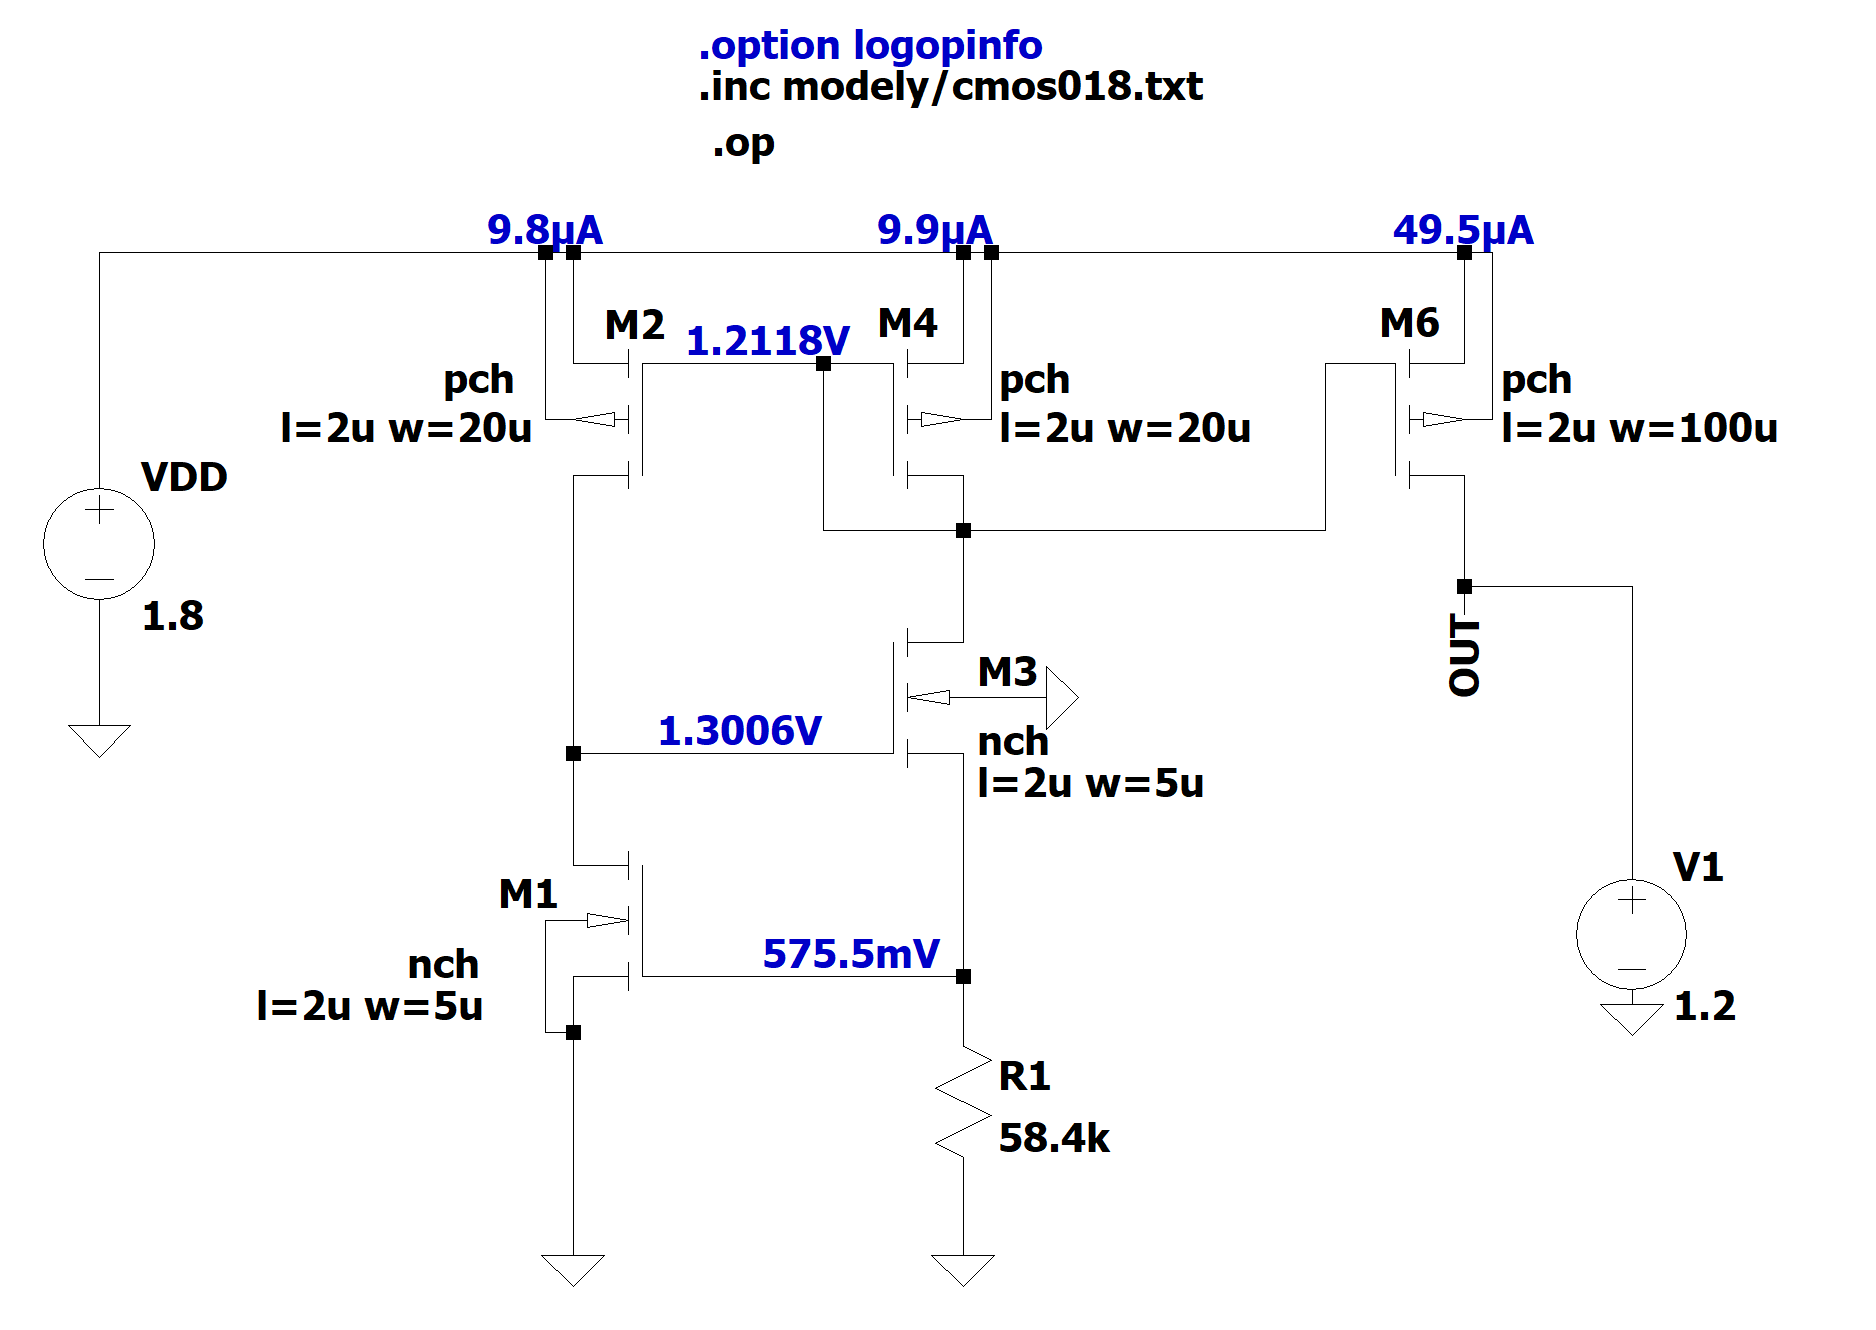
\includegraphics[width=0.9\textwidth]{text/img/PR-op-sch.png}
    \caption{\label{fig:KPZ-op-sch} Zobrazení napětí a proudu ve schématu}
\end{figure}

\vspace{10mm}
\begin{figure}[h!]
    \centering
    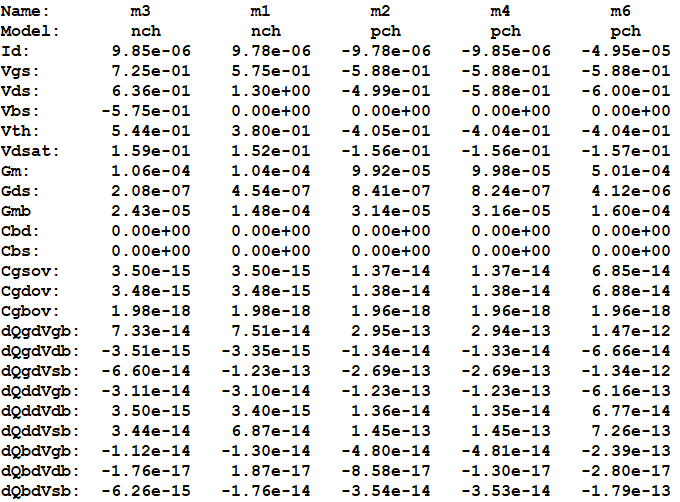
\includegraphics[width=0.9\textwidth]{text/img/PR-op-ol.png}
    \caption{\label{fig:KPZ-op-ol} Pracovní bod tranzistorů}
\end{figure}

